\documentclass[conference]{IEEEtran}
\IEEEoverridecommandlockouts
% The preceding line is only needed to identify funding in the first footnote. If that is unneeded, please comment it out.
\usepackage{cite}
\usepackage[ngerman]{babel}
\usepackage[utf8]{inputenc}
\usepackage{amsmath,amssymb,amsfonts}
\usepackage{algorithmic}
\usepackage{graphicx}
\usepackage{textcomp}
\usepackage{xcolor}
\usepackage{listings}


\definecolor{pblue}{rgb}{0.13,0.13,1}
\definecolor{pgreen}{rgb}{0,0.5,0}
\definecolor{pred}{rgb}{0.9,0,0}
\definecolor{pgrey}{rgb}{0.46,0.45,0.48}
\lstset{language=Java,
	showspaces=false,
	showtabs=false,
	breaklines=true,
	tabsize=2,
	showstringspaces=false,
	breakatwhitespace=true,
	commentstyle=\color{pgreen},
	keywordstyle=\color{pblue},
	stringstyle=\color{pred},
	basicstyle=\ttfamily
}


\usepackage{url}
\def\BibTeX{{\rm B\kern-.05em{\sc i\kern-.025em b}\kern-.08em
		T\kern-.1667em\lower.7ex\hbox{E}\kern-.125emX}}
\begin{document}
	
	\title{Videoanalyse und Objekttracking}
	
	\author{\IEEEauthorblockN{1\textsuperscript{st} Bartolovic Eduard}
		\IEEEauthorblockA{\textit{Hochschule München} \\
			München, Deutschland \\
			eduard.bartolovic0@hm.edu}
	}

	\author{\IEEEauthorblockN{1\textsuperscript{st} Bartolovic Eduard}
		\IEEEauthorblockA{\textit{Hochschule München} \\
			München, Deutschland \\
			eduard.bartolovic0@hm.edu}
	}
	
	\author{\IEEEauthorblockN{1\textsuperscript{st} Bartolovic Eduard}
		\IEEEauthorblockA{\textit{Hochschule München} \\
			München, Deutschland \\
			eduard.bartolovic0@hm.edu}
	}
	
	\maketitle
	
	\begin{abstract}
		
	\end{abstract}
	
	\section{Konzept}
	Ziel des Projektes ist es klassische Verfahren mit neuere DeepLearning Verfahren zu vergleichen.
	Dafür ist für beide arten eine Pipeline geschaffen worden.\\
	Für die Klassische Verfahren wurde für die Objekterkennung Gausmixture verwendet und für das Tracking Sort. Für die DeepLearnig Verfahren wurde für die Objekterkennung ein Neuronales Netz  und für das Tracking wurde Deepsort verwendet.
	
	\begin{figure}[h]
		\begin{center}
			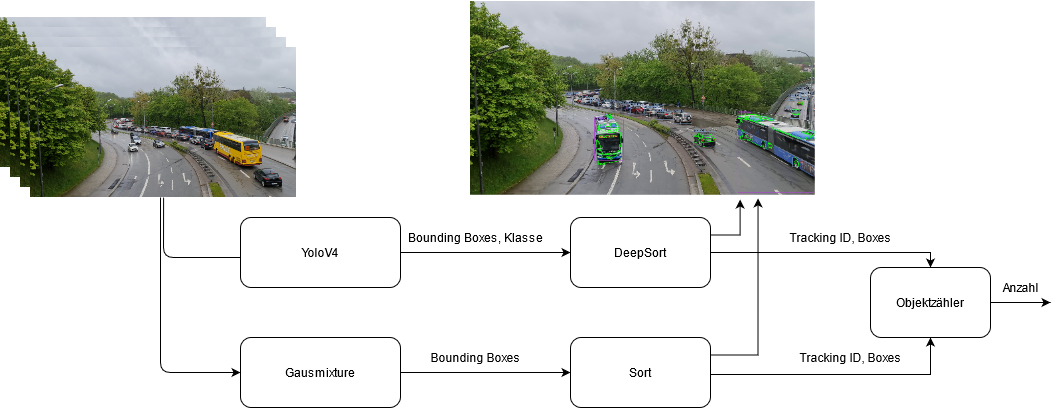
\includegraphics[width=17cm]{Media/KonzeptVAOT.png}
			\caption{Konzept für das Projekt}
			\label{Konzept}
		\end{center}
	\end{figure}
	
	\section{Objekterkennung: Gauß Mixture}
	
	\section{Objekterkennung: YoloV4}
	YOLO ist eine Neuronal Netz für die Echtzeit-Objekterkennung. YOLO ist die Abkürzung für 'You Only Look Once' was übersetzt 'Man sieht nur einmal hin' heißt. Es zerlegt die Aufgabe der Objekterkennung in zwei Teile. Einmal in die Objektposition über Bounding Boxes und dann in Klassifizierung zur Bestimmung der Objektklasse. In diesem Projekt verwendeten wir die 4te Version von Yolo.
	
	\section{Tracking: Sort}
	
	\section{Tracking: DeepSort}
	
	
	\begin{thebibliography}{00}
		\bibitem{b1}www.BlaBla.de
	\end{thebibliography}
	
	
	
	\section{Anhang}
	

\end{document}
